\documentclass[12pt]{article}

\usepackage{complexity}
\usepackage{cmap}
\usepackage[T2A]{fontenc}
\usepackage[utf8]{inputenc}
\usepackage[russian]{babel}
\usepackage{graphicx}
\usepackage{amsthm,amsmath,amssymb}
\usepackage[russian,colorlinks=true,urlcolor=red,linkcolor=blue]{hyperref}
\usepackage{enumerate}
\usepackage{datetime}
\usepackage{minted}
\usepackage{fancyhdr}
\usepackage{lastpage}
\usepackage{color}
\usepackage{verbatim}
\usepackage{tikz}
\usepackage{epstopdf}
\usepackage{enumitem}

\def\THEME{Домашнее задание 1}
\newcommand{\PrE}{\mathbb{E}}
\newcommand{\PrD}{\mathbb{D}}
\newcommand{\PrP}{\mathbb{P}}

\begin{document}

\begin{center}
\vspace*{0mm}
{\LARGE \bf \THEME}
\end{center}

\begin{enumerate}[leftmargin=0pt, rightmargin=0pt]

\item

\begin{enumerate}[leftmargin=20pt, rightmargin=0pt, itemsep=7pt]

\item

И браузер, и сервер используют \texttt{HTTP 1.1}.

\item

\texttt{ru-RU, ru, en-US, en}. Дополнительно сообщается версия браузера, операционная система пользователя, возможные файлы, которые может принять клиент.

\item

Клиент - 192.168.0.171. Сервер - 128.119.245.12.

\item

\texttt{200 OK}.

\item

Sat, 26 Feb 2022 06:59:01 GMT.

\item

128.

\end{enumerate}

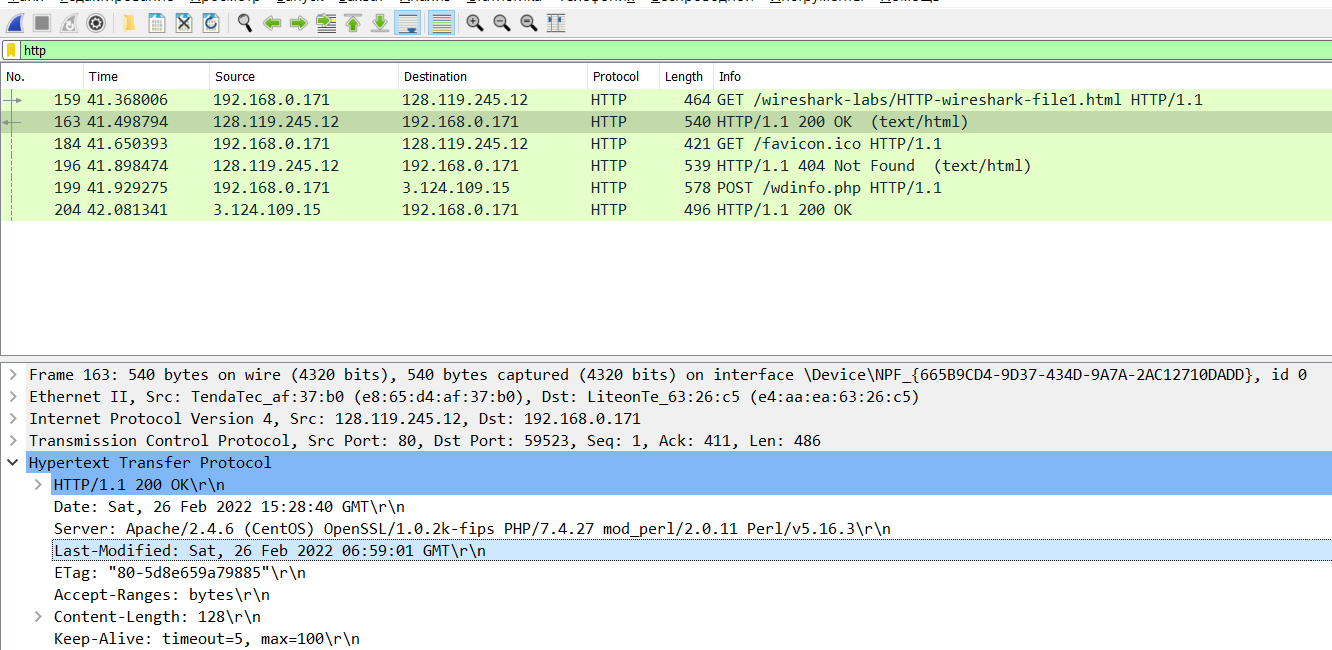
\includegraphics[scale=0.5]{1.1.png}

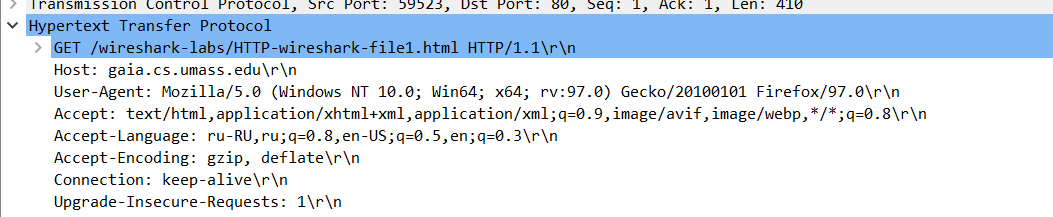
\includegraphics[scale=0.5]{1.2.png}

\item

\begin{enumerate}[leftmargin=20pt, rightmargin=0pt, itemsep=7pt]

\item

Нет.

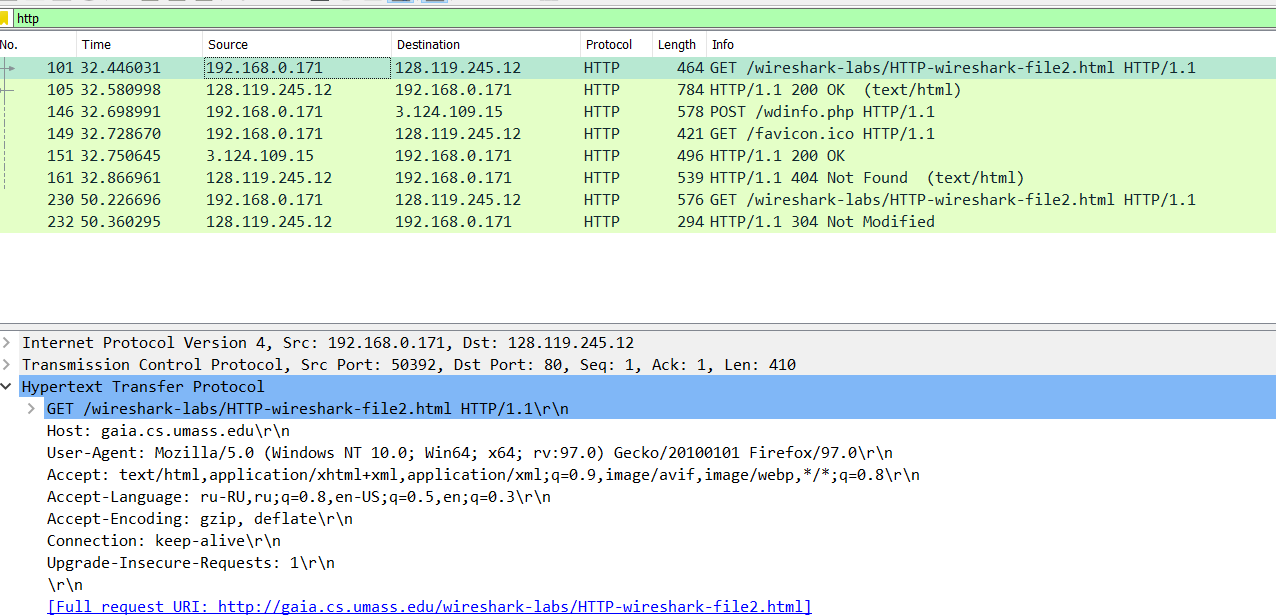
\includegraphics[scale=0.5]{2.1.png}

\item

Да. Ответ отображается в поле \texttt{Line-based text data}.

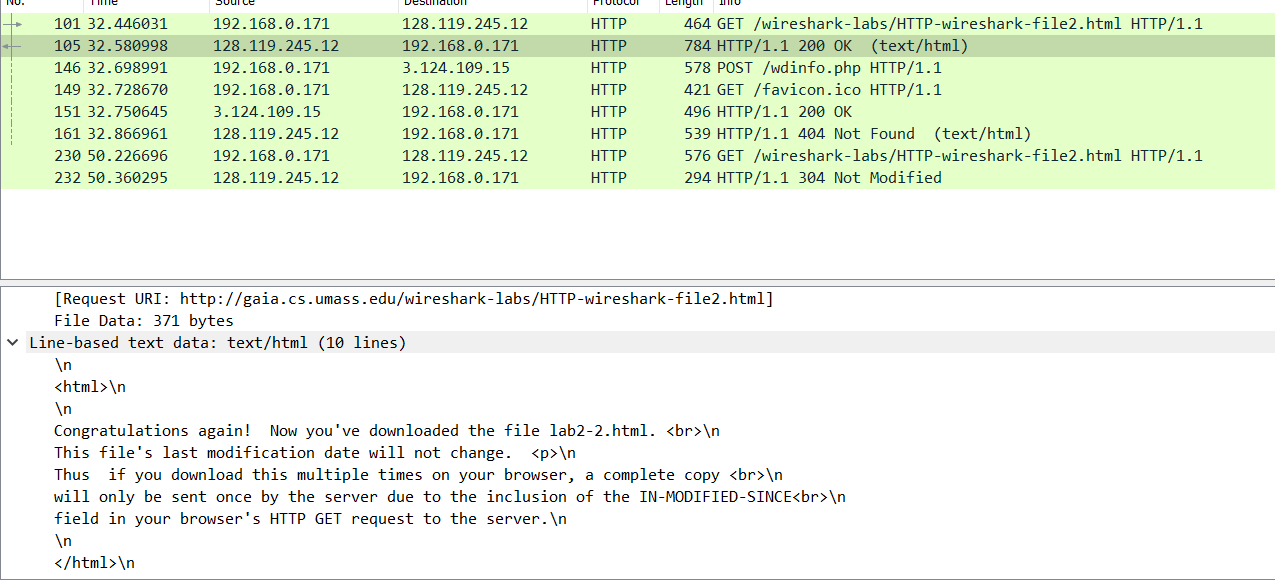
\includegraphics[scale=0.5]{2.2.png}

\item

Да, за ним следует дата, когда файл последний раз обновлялся на сервере. Соответственно, если дата не изменилась, то возвращается закэшированный браузером файл.

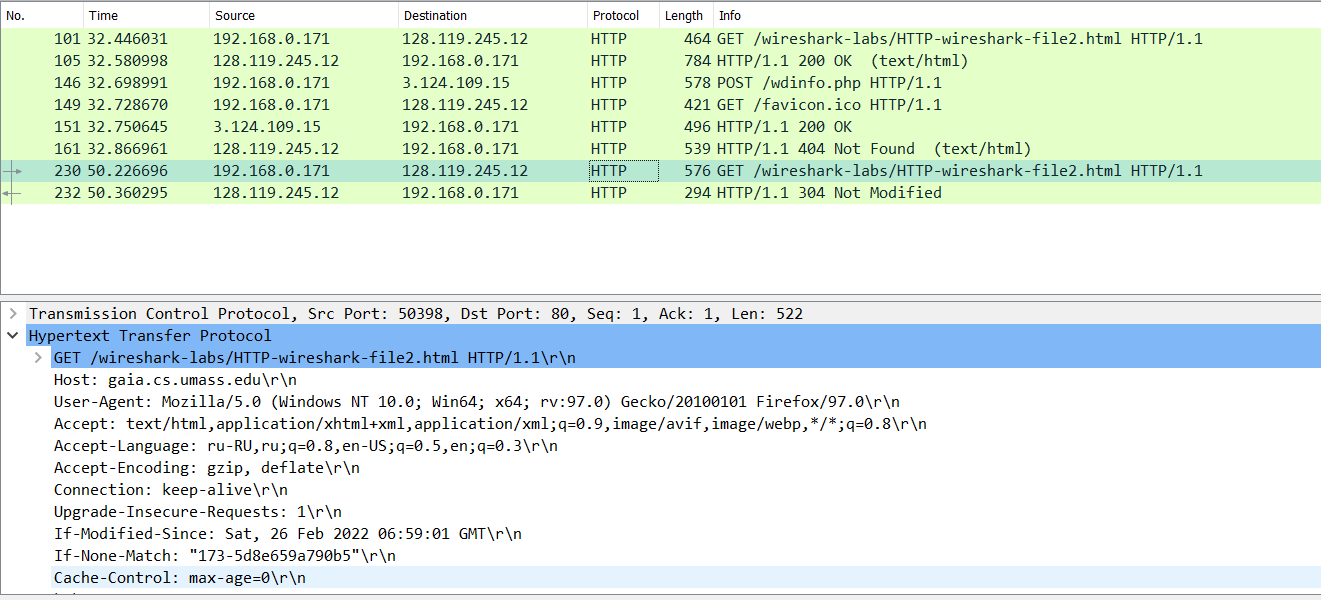
\includegraphics[scale=0.5]{2.3.png}

\item

\texttt{304 Not Modified}. Явно файл не вернул.

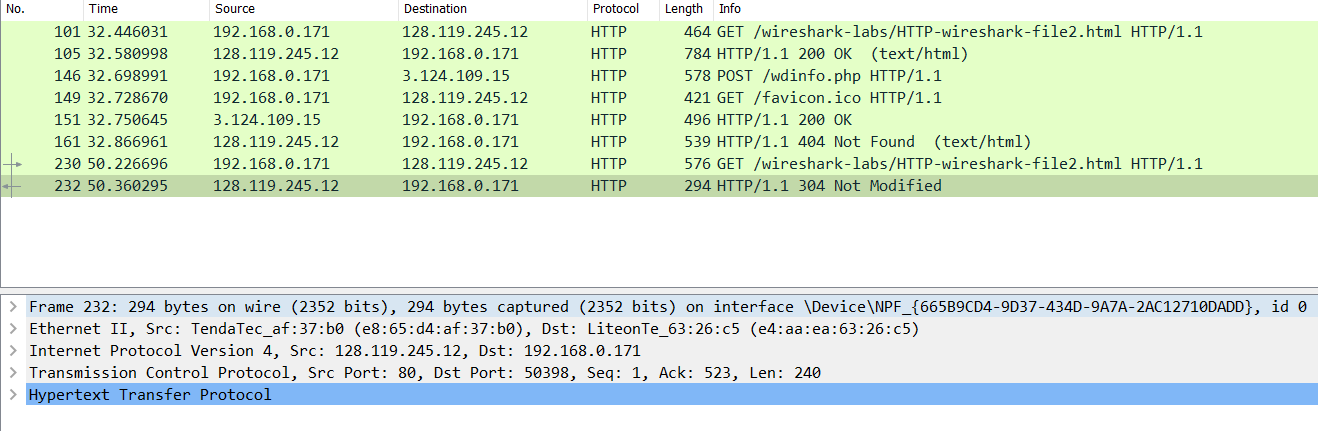
\includegraphics[scale=0.5]{2.4.png}

\end{enumerate}

\item

\begin{enumerate}[leftmargin=20pt, rightmargin=0pt, itemsep=7pt]

\item

Два. Пакет №15.

\item

№22.

\item

Четыре.

\item

Нет.

\end{enumerate}

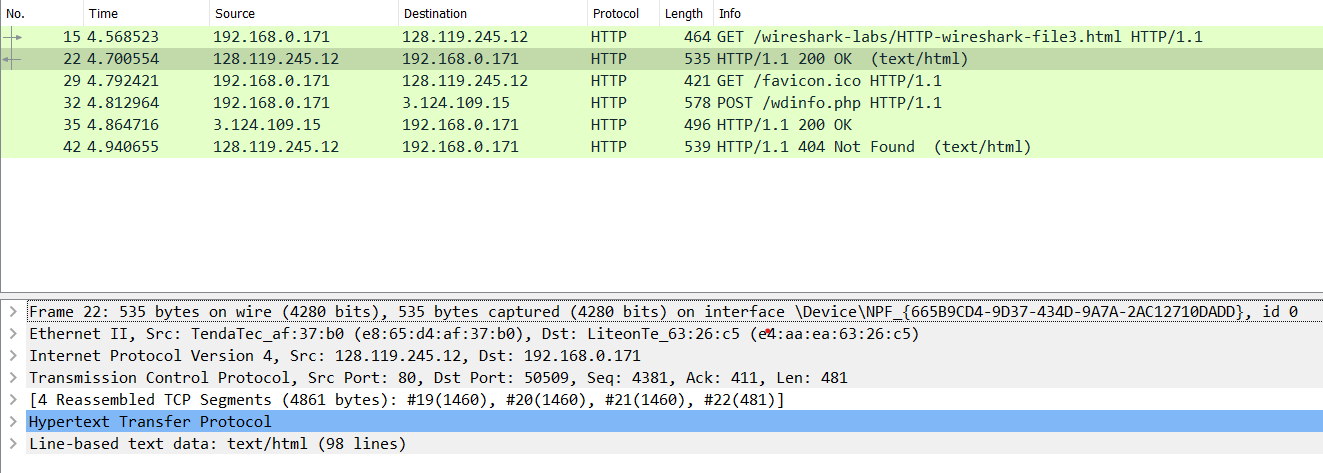
\includegraphics[scale=0.5]{3.1.png}

\item

\begin{enumerate}[leftmargin=20pt, rightmargin=0pt, itemsep=7pt]

\item

Четыре \texttt{GET} запроса на адреса \texttt{128.119.245.12} и \texttt{178.79.137.164}.

\item

Картинки загружались параллельно, потому что запрос \texttt{GET} для второй картинки случился раньше, чем пришёл ответ на запрос \texttt{GET} для первой картинки.

\end{enumerate}

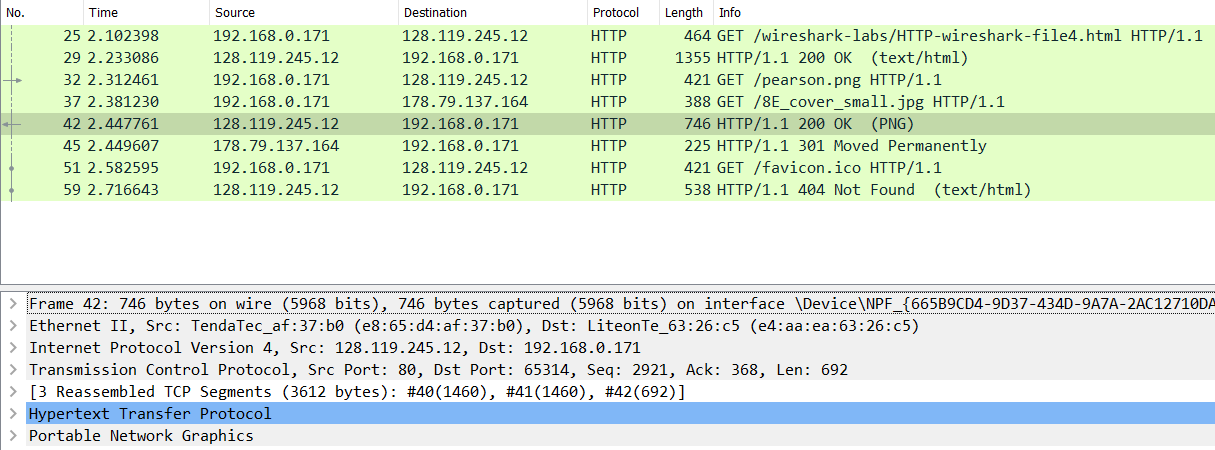
\includegraphics[scale=0.5]{4.1.png}

\item

\begin{enumerate} [leftmargin=20pt, rightmargin=0pt, itemsep=7pt]

\item

\texttt{401 Unauthorized.}

\item

Появилось поле \texttt{Credentials} с логином и паролем.

\end{enumerate}

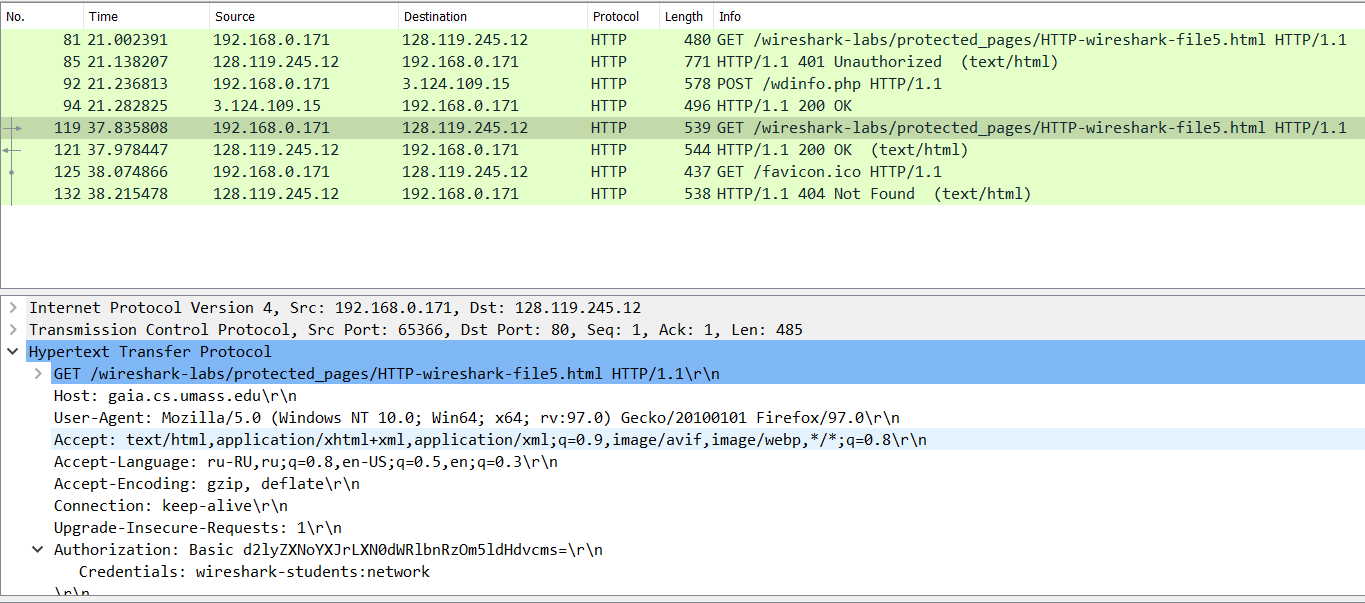
\includegraphics[scale=0.5]{5.1.png}

\end{enumerate}

\end{document}